\documentclass[12pt, twoside]{article}
\usepackage[utf8]{inputenc}
\usepackage[english,russian]{babel}
\newcommand{\hdir}{.}

\usepackage{graphicx}
\usepackage{caption}
\usepackage{amssymb}
\usepackage{mathrsfs}
\usepackage{euscript}
\usepackage{upgreek}
\usepackage{array}
\usepackage{theorem}
\usepackage{graphicx}
\usepackage{subfig}
\usepackage{caption}
\usepackage{color}
\usepackage{url}
\usepackage{amsmath, bm}

\usepackage{cancel}

\DeclareMathOperator*{\argmax}{arg\,max}
\DeclareMathOperator*{\argmin}{arg\,min}

\usepackage[left=2cm, right=2cm, top=3cm, bottom=3cm, bindingoffset=0cm]{geometry}

\newcommand{\Pb}{\mathcal{P}}

\setcounter{secnumdepth}{-1}

\begin{document} 

\title{Задание 4 по курсу "Байесовский выбор модели"}
\author{Грабовой Андрей, группа 574}
\date{}
\maketitle

\section{Задача}

Рассмотрим вероятностную модель метода главных компонент, считая, что 
$$\forall\textbf{x} \in \mathbb{R}^{n}~\exists\textbf{z} \in \mathbb{R}^{d}:~\textbf{x}=\textbf{W}\textbf{z}+ \bm{\mu} +\bm{\varepsilon}, \eqno(1)$$
где $\bm{\mu}\in\mathbb{R}^{n},~\bm{\varepsilon}\in\mathbb{R}^{n}$.

Пусть имеется iid выборка  $\textbf{X} = [\textbf{x}_1, \cdots, \textbf{x}_{m}]$. Пусть:
$$p(\textbf{z}) = N(\textbf{z}|\textbf{0}, \textbf{I}),\quad p(\bm{\varepsilon})=N(\bm{\varepsilon}|\textbf{0}, \sigma^2\textbf{I}).\eqno(2)$$

\paragraph{a)}
$$p(\textbf{X}, \textbf{Z}|\textbf{W}, \bm{\mu}, \sigma) = \prod_{i=1}^{m}N(\textbf{x}_{i}|\textbf{W}\textbf{z}_{i}+\bm{\mu}, \sigma^2\textbf{I})\prod_{i=1}^{m}N(\textbf{z}_{i}|\textbf{0}, \textbf{I}). \eqno(3)$$

\paragraph{б)} 
$$p(\textbf{X}|\textbf{W}, \bm{\mu}, \sigma) = \prod_{i=1}^{m}N(\textbf{x}_{i}|\bm{\mu}, \textbf{W}\textbf{W}^{\mathsf{T}}+\sigma^2\textbf{I}). \eqno(4)$$

\paragraph{в)} Используя $EM$-алгоритм решим задачу максимизации обоснованности:
$$F(q, \textbf{W}, \bm{\mu}, \sigma) = \log p(\textbf{X}|\textbf{W}, \bm{\mu}, \sigma) - \sum_{i=1}^{m}D_{KL}(q(\textbf{z}_i)||p(\textbf{z}_i|\textbf{x}_i,\textbf{W},\bm{\mu},\sigma)).\eqno(5)$$

Очевидно, что $E$-шаг имеет следующее решение:
$$q(\textbf{z}_i) = p(\textbf{z}_i|\textbf{x}_i,\textbf{W},\bm{\mu},\sigma),\eqno(6)$$
где апостериорное распределение на $\textbf{z}_i$ является нормальным, так как правдоподобие является нормальным. Тогда апостериорное распределение будет иметь параметры(по аналогии с прошлой домашкой) получаем:
$$q(\textbf{z}_i) = N(\textbf{z}_i|\textbf{m}_i, \textbf{A}) \quad \textbf{A} = \left(\frac{1}{\sigma^2}\textbf{W}^{\mathsf{T}}\textbf{W}+\textbf{I}\right)^{-1} \quad \textbf{m}_i = \frac{1}{\sigma^2}\textbf{A}\textbf{W}^{\mathsf{T}}(\textbf{x}_i - \bm{\mu}). \eqno(7)$$

Найдем итеративные формулы для $M$-шага, для этого запишем:
$$\mathsf{E}_{q(\textbf{Z})}\log p(\textbf{X},\textbf{Z}|\textbf{W}, \bm{\mu}, \sigma) = \mathcal{F}(\textbf{W}, \bm{\mu}, \sigma) = $$
$$= \sum_{i=1}^{m}\mathsf{E}_{q(\textbf{Z})}\left( -\frac{1}{2}\textbf{z}_{i}^{\mathsf{T}}\textbf{z}_{i}-\frac{1}{2\sigma^2}\left(\textbf{W}\textbf{z}_i+\bm{\mu}-\textbf{x}_i\right)^{\mathsf{T}}\left(\textbf{W}\textbf{z}_i+\bm{\mu}-\textbf{x}_i\right)-\frac{n}{2}\log\sigma^2\right)-\frac{m\left(d+n\right)}{2}\log2\pi. \eqno(8)$$

$$\frac{\partial \mathcal{F}}{\partial \bm{\mu}} = \frac{1}{\sigma^2}\sum_{i=1}^{m}\mathsf{E}\left(\textbf{W}\textbf{z}_{i}+\bm{\mu}-\textbf{x}_i\right) = 0 \Rightarrow \bm{\mu} = \frac{1}{m}\sum_{i=1}^{m}\left(\textbf{x}_i - \textbf{W}\mathsf{E}\textbf{z}_i\right) \Rightarrow \bm{\mu} = \frac{1}{m}\sum_{i=1}^{m}\textbf{x}_i. \eqno(9)$$

$$\frac{\partial \mathcal{F}}{\partial \textbf{W}} = \sum_{i=1}^{m}\mathsf{E}\left( \textbf{W}\textbf{z}_i +\bm{\mu} - \textbf{x}_i \right)\textbf{z}_i^{\mathsf{T}} = \sum_{i=1}^{m}\left(\textbf{W}\mathsf{E}\textbf{z}_i\textbf{z}_i^{\mathsf{T}} + (\bm{\mu} - \textbf{x}_i)\mathsf{E}\textbf{z}_i^{\mathsf{T}} \right) \Rightarrow$$
$$\Rightarrow \textbf{W}_{new} = \left(\sum_{i=1}^{m}(\textbf{x}_i - \bm{\mu}_{new})\mathsf{E}\textbf{z}_i^{\mathsf{T}}\right)\left(\sum_{i=1}^{m}\mathsf{E}\textbf{z}_i\textbf{z}_i^{\mathsf{T}}\right)^{-1}, \eqno(10)$$

$$\frac{\partial \mathcal{F}}{\partial \sigma^2} = \frac{1}{2\sigma^4}\sum_{i=1}^{m}\mathsf{E}\left(\textbf{W}\textbf{z}_i+\bm{\mu}-\textbf{x}_i\right)^{\mathsf{T}}\left(\textbf{W}\textbf{z}_i+\bm{\mu}-\textbf{x}_i\right) - \frac{n\cdot m}{2\sigma^2}=0\Rightarrow$$
$$\Rightarrow \sigma^2_{new} = \frac{1}{nm}\sum_{i=1}^{m}\left(\mathsf{E}\textbf{z}_i^{\mathsf{T}}\textbf{W}_{new}^{\mathsf{T}}\textbf{W}_{new}\textbf{z}_i + \left(\bm{\mu}_{new} - \textbf{x}_i\right)^{\mathsf{T}}\left(\bm{\mu}_{new} - \textbf{x}_i\right) + 2\mathsf{E}\textbf{z}_{i}^{\mathsf{T}}\textbf{W}_{new}^{\mathsf{T}}\left(\bm{\mu}_{new}-\textbf{x}_i\right)\right), \eqno(11)$$

где в (10) и в (11) $\mathsf{E}\textbf{z}_i$ и $\mathsf{E}\textbf{z}_i\textbf{z}_i^{\mathsf{T}}$ очевидно определяються из (7), первое слагаемое суммы расписывается через след и тоже выделяется математическое ожидание от $\mathsf{E}\textbf{z}_i\textbf{z}_i^{\mathsf{T}}$.\\

Пусть теперь в данных могут быть пропуски.
Тогда каждый вектор $\textbf{x}^n$ можно условно разбить на два подвектора $\textbf{x}^{n}_{\text{obs}}$ и $\textbf{x}^{n}_{miss}$. Тогда формально матрица $\textbf{X}$ разбивается на две матрицы $\textbf{X}_{obs}$ и $\textbf{X}_{miss}$. Тогда правдоподобие модели выглядит следующим образом:
$$p(\textbf{X}_{obs}, \textbf{X}_{miss}, \textbf{T}|\textbf{W}, \bm{\mu}, \sigma) = \prod_{i=1}^{m}N(\textbf{x}^{i}_{obs}|\textbf{W}_{obs}\textbf{z}_{i} + \bm{\mu}_{obs}, \sigma^2\textbf{I})N(\textbf{x}^{i}_{miss}|\textbf{W}_{miss}\textbf{z}_{i} + \bm{\mu}_{miss}, \sigma^2\textbf{I})N(\textbf{z}_i|\textbf{0}, \textbf{I}),\eqno(12)$$
проще говоря все изменения состоят в том, что в нас теперь имеется не по одному $\bm{\mu}$, $\textbf{W}$, а по два экземпляра, для случая если признак пропущен и если признак наблюдается.

Модификация $EM$-алгоритма будет в том, что в качестве скрытых переменных, теперь не только $\textbf{z}$, но и пропущенные значения $\textbf{x}_{miss}$. Тоесть теперь в формуле (6) появится еще и и $\textbf{x}_{miss}$, тоесть:
$$q(\textbf{z}_{i}, \textbf{x}^{i}_{miss}) = p\left((\textbf{z}_i, \textbf{x}^{i}_{miss})|\textbf{W}, \bm{\mu}, \sigma\right) = N\left((\textbf{z}_i, \textbf{x}^{i}_{miss})|\textbf{m}_i, \textbf{A}_i\right), \eqno(13)$$
дальше используя свойство сопряжения можно найти $\textbf{m}_i$, $\textbf{A}_i$ и повторяя теже самые действия можно выписать итеративные формулы.

\paragraph{г)} 

\begin{figure}[h!]\center
{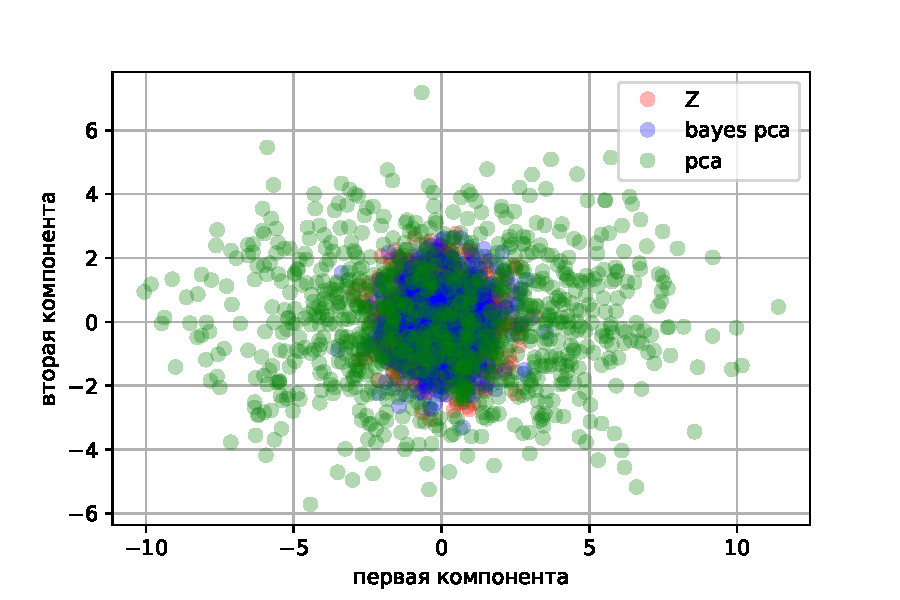
\includegraphics[width=0.8\textwidth]{Task4_1}}
\caption{Изображение латентного пространства}
\label{Task4_1}
\end{figure}

На рис.~\ref{Task4_1}  показано изображение скрытого пространства, истинного, через простой PCA и через Bayes PCA.   Как видно из рисунка bayes PCA и истинные вектора Z имеют одинаковые распределение, тоесть он полностью восстановил истинное скрытое пространство.

\paragraph{д)} 

Теперь опишем метод автоматического определения числа компонент.

$$p(\textbf{W}|\alpha) = \prod_{i=1}^{n}\sqrt{\frac{\alpha_i}{2\pi}}^{n}\exp\left(-\frac{\alpha_i}{2}\textbf{w}_i^{\mathsf{T}}\textbf{w}_i\right). \eqno(14)$$

Правдоподобие:

$$p(\textbf{X}, \textbf{Z}, \textbf{W}|\bm{\mu}, \bm{\alpha}, \sigma)=p(\textbf{X}|\textbf{Z}, \textbf{W}, \bm{\mu}, \bm{\alpha}, \sigma)p(\textbf{Z})p(\textbf{W}|\bm{\alpha}). \eqno(15)$$

Будем искать решение $E$-шага в следующем виде:
 $$q(\textbf{W}, \textbf{z}_1,\cdots,\textbf{z}_m) = q(\textbf{W}) \prod_{i=1}^{m} q(\textbf{z}_i). \eqno(16)$$

$$\log q(\textbf{z}_i) = \mathsf{E}_{q/z_i}\log p(\textbf{X}, \textbf{Z}, \textbf{W}|\bm{\mu}, \bm{\alpha}, \sigma)\propto$$
$$\propto -\frac{1}{2}\mathsf{E}_{q/z_i}\left(\textbf{z}_i^{\mathsf{T}}\textbf{z}_i + \frac{1}{\sigma^2}\left[\textbf{W}\textbf{z}_i+\bm{\mu} - \textbf{x}_i\right]^{\mathsf{T}}\left[\textbf{W}\textbf{z}_i+\bm{\mu} - \textbf{x}_i\right]\right) = $$
$$ = -\frac{1}{2}\left[\textbf{z}_i^{\mathsf{T}}\left(\textbf{I} +\frac{1}{\sigma^2}\mathsf{E}_{\textbf{W}}\textbf{W}^{\mathsf{T}}\textbf{W} \right)\textbf{z}_i +2\frac{1}{\sigma^2}\textbf{z}_i^{\mathsf{T}}\mathsf{E}_{\textbf{W}}\textbf{W}^{\mathsf{T}}(\bm{\mu} - \textbf{x}_i)\right], \eqno(17)$$
из (17) получаем, что:
$$q(\textbf{z}_i) = N(\textbf{z}_i|\textbf{m}_i, \textbf{A}) \quad \textbf{A} = \left(\frac{1}{\sigma^2}\mathsf{E}\textbf{W}^{\mathsf{T}}\textbf{W}+\textbf{I}\right)^{-1} \quad \textbf{m}_i = \frac{1}{\sigma^2}\textbf{A}\mathsf{E}\textbf{W}^{\mathsf{T}}(\textbf{x}_i - \bm{\mu}), \eqno(18)$$
то есть получили здесь тоже самое, что и в (7).

$$\log q(\textbf{W}) = \mathsf{E}_{q/W}\log p(\textbf{X}, \textbf{Z}, \textbf{W}|\bm{\mu}, \bm{\alpha}, \sigma)\propto$$
$$ \propto \mathsf{E}_{q/W}\left(-\frac{1}{2\sigma^2}\sum_{i=1}^{m}\left[\textbf{W}\textbf{z}_i +\bm{\mu} - \textbf{x}_i\right]^{\mathsf{T}}\left[\textbf{W}\textbf{z}_i +\bm{\mu} - \textbf{x}_i\right] -\frac{1}{2}\sum_{j=1}^{n}\textbf{w}_j^{\mathsf{T}}\textbf{w}_j\right) \propto $$
$$ \propto -\frac{1}{2\sigma^2}\sum_{i=1}^{m}\left(\mathsf{E}_{q/W} \textbf{z}_i^{\mathsf{T}}\textbf{W}^{\mathsf{T}}\textbf{W}\textbf{z}_i + 2\textbf{m}_i^{\mathsf{T}}\textbf{W}^{\mathsf{T}}(\bm{\mu} - \textbf{x}_i) \right) - \frac{1}{2}\sum_{j=1}^{n}\alpha_j\textbf{w}_j^{\mathsf{T}}\textbf{w}_j = $$
$$ = -\frac{1}{2}\left[\frac{1}{\sigma^2}\sum_{i=1}^{m}\textbf{tr}\left(\textbf{W}\mathsf{E}\textbf{z}_i\textbf{z}_i^{\mathsf{T}}\textbf{W}^{\mathsf{T}}\right) + \sum_{j=1}^{n}\alpha_j\textbf{w}_j^{\mathsf{T}}\textbf{w}_j\right] -\frac{1}{2}\left[2\frac{1}{\sigma^2}\sum_{i=1}^{m}\textbf{tr}\left((\bm{\mu}-\textbf{x}_i)\textbf{m}_i^{\mathsf{T}}\textbf{W}^{\mathsf{T}}\right)\right]=$$
$$ = -\frac{1}{2}\textbf{tr}\left(\textbf{W}^{\mathsf{T}}\frac{1}{\sigma^2}\sum_{i=1}^{m}\mathsf{E}\textbf{z}_i\textbf{z}_i^{\mathsf{T}}\textbf{W} + \textbf{W}^{\mathsf{T}}\text{diag}(\bm{\alpha})\textbf{W}\right) -\frac{1}{2}\left[2\frac{1}{\sigma^2}\sum_{i=1}^{m}\textbf{tr}\left((\bm{\mu}-\textbf{x}_i)\textbf{m}_i^{\mathsf{T}}\textbf{W}^{\mathsf{T}}\right)\right]=$$
$$ = -\frac{1}{2}\textbf{tr}\left(\textbf{W}^{\mathsf{T}}\frac{1}{\sigma^2}\sum_{i=1}^{m}\mathsf{E}\textbf{z}_i\textbf{z}_i^{\mathsf{T}} + \text{diag}(\bm{\alpha})\textbf{W}\right) -\frac{1}{2}\left[2\frac{1}{\sigma^2}\sum_{i=1}^{m}\textbf{tr}\left((\bm{\mu}-\textbf{x}_i)\textbf{m}_i^{\mathsf{T}}\textbf{W}^{\mathsf{T}}\right)\right]=$$
$$ = -\frac{1}{2}\left[\sum_{j=1}^{n}\textbf{w}_j^{\mathsf{T}}\textbf{B}_j^{-1}\textbf{w}_j -2\sum_{j=1}^{n}\textbf{w}_j^{\mathsf{T}}\textbf{B}_j^{-1}\textbf{u}_j\right], \eqno(19)$$
 где введены обозначения:
 $$\textbf{B}^{-1}_j = \left(\frac{1}{\sigma^2}\sum_{i=1}^{m}\mathsf{E}\textbf{z}_i\textbf{z}_i^{\mathsf{T}} + \text{diag}(\bm{\alpha})\right) \quad \textbf{u}_j = \textbf{B}_j\left(\frac{1}{\sigma^2}\sum_{i=1}^{m} (\textbf{x}_i - \bm{\mu})\textbf{m}_i^{\mathsf{T}} \right)_j, \eqno(20)$$
где под выражением $\left(\cdots\right)_j$ подрозумевается взятие $j$-го столбца матрицы. Тогда из (19) получаем, что:
$$q(\textbf{w}_j) = N(\textbf{w}_{j}|\textbf{u}_j, \textbf{B}_j), \eqno(21)$$
где $\textbf{u}$ и $\textbf{B}$ определяются формулой (20).

На этом мы закончили делать $E$-шаг. Теперь нужно сделать $M$-шаг.

$$ \mathsf{E}_{q(\textbf{Z}, \textbf{W})}\log p(\textbf{X}, \textbf{Z}, \textbf{W}|\bm{\mu}, \bm{\alpha}, \sigma) = \mathcal{F}(\bm{\mu}, \bm{\alpha}, \sigma) = $$
$$ = \frac{1}{2\sigma^2}\sum_{i=1}^{m}\mathsf{E}\left[\textbf{X}\textbf{z}_i + \bm{\mu} - \textbf{x}_i\right]^{\mathsf{T}}\left[\textbf{X}\textbf{z}_i + \bm{\mu} - \textbf{x}_i\right] - \frac{1}{2}\sum_{j=1}^{n}\alpha_j\textbf{w}_j^{\mathsf{T}}\textbf{w}_j-\frac{n\cdot m}{2}\log\sigma^2 + \frac{d}{2}\sum_{j=1}^{n}\log{\alpha_j}. \eqno(22)$$

$$\frac{\partial\mathcal{F}}{\partial\bm{\mu}} =  \frac{1}{\sigma^2}\sum_{i=1}^{m}\mathsf{E}\left(\textbf{W}\textbf{z}_{i}+\bm{\mu}-\textbf{x}_i\right) = 0 \Rightarrow \bm{\mu}^{new} = \frac{1}{m}\sum_{i=1}^{m}\textbf{x}_i - \frac{1}{m}\mathsf{E}\textbf{W}\sum_{i=1}^{m}\mathsf{E}\textbf{z}_i , \eqno(23)$$

$$\frac{\partial\mathcal{F}}{\partial\alpha_j} = -\frac{1}{2}\mathsf{E}\textbf{w}_j^{\mathsf{T}}\textbf{w}_j + \frac{d}{2\alpha_j} = 0 \Rightarrow \alpha_j^{new}  = \frac{d}{\mathsf{E}\textbf{w}_j^{\mathsf{T}}\textbf{w}_j}, \eqno(24)$$

$$\frac{\partial\mathcal{F}}{\partial\sigma^2} = \frac{1}{2\sigma^4}\sum_{i=1}^{m}\mathsf{E}\left(\textbf{W}\textbf{z}_i+\bm{\mu} - \textbf{x}_i\right)^{\mathsf{T}}\left(\textbf{W}\textbf{z}_i+\bm{\mu} - \textbf{x}_i\right) - \frac{m\cdot n}{2\sigma^2} = 0 \Rightarrow $$
$$\Rightarrow \sigma^2_{new} = \frac{1}{n\cdot m}\sum_{i=1}^{m}\left[ \mathsf{E}\left(\textbf{z}_i^{\mathsf{T}}\textbf{W}^{\mathsf{T}}\textbf{W}\textbf{z}_i\right) + \left(\bm{\mu}^{new}-\textbf{x}_i\right)^{\mathsf{T}}\left(\bm{\mu}^{new}-\textbf{x}_i\right) + 2\mathsf{E}\left(\textbf{z}_i^{\mathsf{T}}\right)\mathsf{E}\left(\textbf{W}^{\mathsf{T}}\right)\left(\bm{\mu}^{new} - \textbf{x}_i\right) \right], \eqno(25)$$
где $\mathsf{E}\textbf{W}$, $\mathsf{E}\textbf{w}_{j}^{\mathsf{T}}\textbf{w}_j$,  $\mathsf{E}\textbf{z}_i$, $\mathsf{E}\textbf{z}_{j}\textbf{z}_j^{\mathsf{T}}$, $\mathsf{E}\textbf{W}^{\mathsf{T}}\textbf{W}$ легко находятся из формул (18), (20), (21):
$$\mathsf{E}\textbf{W} = \left(\sum_{i=1}^{m}\left(\textbf{x}_i-\bm{\mu}\right)\textbf{m}_i^{\mathsf{T}}\right)\left(\sum_{i=1}^{m}\textbf{z}_i\textbf{z}_i^{\mathsf{T}} + \sigma^2\text{diag}(\bm{\alpha})\right)^{-1}, \eqno(26)$$

$$\mathsf{E}\textbf{w}_j^{\mathsf{T}}\textbf{w}_j = \textbf{tr}\left(\textbf{B}_j+\textbf{u}_j\textbf{u}_j^{\mathsf{T}}\right), \eqno(27)$$
$$\mathsf{E}\textbf{z}_j = \textbf{m}_j, \eqno(28)$$

$$\mathsf{E}\textbf{z}_j^{\mathsf{T}}\textbf{z}_j = \textbf{tr}\left(\textbf{A}+\textbf{m}_j\textbf{m}_j^{\mathsf{T}}\right), \eqno(29)$$

$$\mathsf{E}\textbf{W}^{\mathsf{T}}\textbf{W} = \text{diag}(\mathsf{E}\textbf{w}_i^{\mathsf{T}}\textbf{w}_i), \eqno(30)$$

Получили итеративные формулы для решения задачи.

\paragraph{e)}

\begin{figure}[h!]\center
{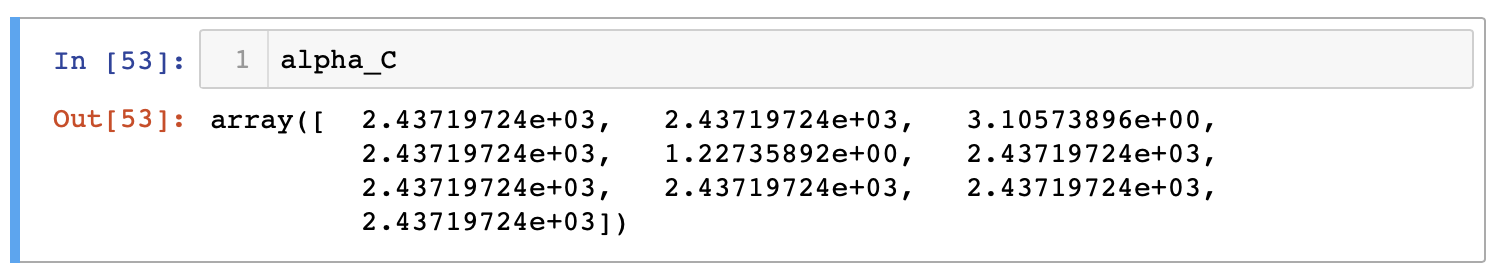
\includegraphics[width=0.8\textwidth]{Task4_3}}
\caption{Таблица результатов для $\alpha$}
\label{Task4_2}
\end{figure}

На рис.~\ref{Task4_2} показана таблица, результата работы алгоритма из пункта д). Как видно из результатов, алгоритм сократил количество компонент до 2, как и предполагалось. Это следует из того, что все $\alpha$ кроме 2 очень большие $\approx10^3$, в то время как $3$ и $5$ компоненты вектора $\alpha$ порядка единиц.




\end{document} 